\documentclass{beamer}
\usepackage[latin1]{inputenc}
\usetheme{boxes}
\title[defaultdict]{defaultdict tutorial}
\author{Michelle Fullwood}
\date{}
\usepackage{color}
\newsavebox{\mysavebox}
\usepackage{listings}

\usepackage{verbdef}

\definecolor{mygreen}{rgb}{0,0.6,0}
\definecolor{mygray}{rgb}{0.5,0.5,0.5}
\definecolor{mymauve}{rgb}{0.58,0,0.82}

\lstset{ %
  backgroundcolor=\color{white},   % choose the background color; you must add \usepackage{color} or \usepackage{xcolor}
  basicstyle=\ttfamily\normalsize,        % the size of the fonts that are used for the code
  keywordstyle=\bfseries,
  identifierstyle=\color{red},     % object names
  commentstyle=\rmfamily\itshape, % italic comments
  stringstyle=\slshape,           % strings
  breakatwhitespace=false,         % sets if automatic breaks should only happen at whitespace
  breaklines=true,                 % sets automatic line breaking
  captionpos=b,                    % sets the caption-position to bottom
  commentstyle=\color{mygreen},    % comment style
  deletekeywords={...},            % if you want to delete keywords from the given language
  escapeinside={\%*}{*)},          % if you want to add LaTeX within your code
  extendedchars=true,              % lets you use non-ASCII characters; for 8-bits encodings only, does not work with UTF-8
  frame=none, %single,                    % adds a frame around the code
  keepspaces=true,                 % keeps spaces in text, useful for keeping indentation of code (possibly needs columns=flexible)
  keywordstyle=\color{blue},       % keyword style
  language=Python,                 % the language of the code
  morekeywords={*,^,...},            % if you want to add more keywords to the set
  numbers=none,                    % where to put the line-numbers; possible values are (none, left, right)
  numbersep=5pt,                   % how far the line-numbers are from the code
  numberstyle=\tiny\color{mygray}, % the style that is used for the line-numbers
  rulecolor=\color{black},         % if not set, the frame-color may be changed on line-breaks within not-black text (e.g. comments (green here))
  showspaces=false,                % show spaces everywhere adding particular underscores; it overrides 'showstringspaces'
  showstringspaces=false,          % underline spaces within strings only
  showtabs=false,                  % show tabs within strings adding particular underscores
  stepnumber=2,                    % the step between two line-numbers. If it's 1, each line will be numbered
  stringstyle=\color{mymauve},     % string literal style
  tabsize=2,                       % sets default tabsize to 2 spaces
%  title=\lstname                   % show the filename of files included with \lstinputlisting; also try caption instead of title
}



\begin{document}

\begin{frame}
\titlepage
\end{frame}

\begin{frame}{Motivation}
 Common task in text processing: doing a frequency count.
 
 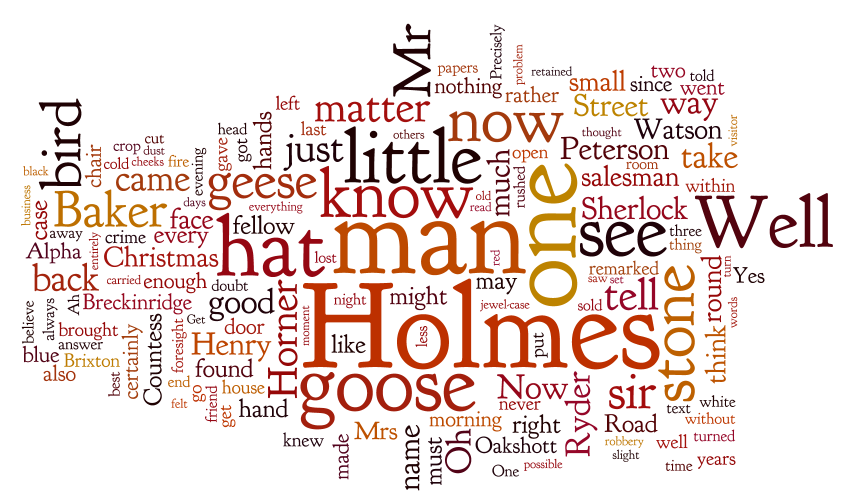
\includegraphics[scale=0.35]{holmes_wordle.png} 
\end{frame}

\begin{lrbox}{\mysavebox}
\begin{lstlisting}
# frequency count for words in some text

text = "baa baa black sheep".split()

freqcount = dict()
for word in text:
    if word not in freqcount:
        freqcount[word] = 0
    freqcount[word] += 1

print freqcount

# {'sheep': 1, 'black': 1, 'baa': 2}

\end{lstlisting}
\end{lrbox}

\begin{frame}{Common pattern}
\vspace{1.5em}
{\usebox{\mysavebox}}
\vspace{1em}
\end{frame}


\begin{lrbox}{\mysavebox}
\begin{lstlisting}
# frequency count for words in some text

text = "baa baa black sheep".split()

from collections import defaultdict
freqcount = defaultdict(int)
for word in text:
    freqcount[word] += 1

print freqcount
# defaultdict(<type 'int'>, {'sheep': 1, 'black': 1, 'baa': 2})
\end{lstlisting}

\end{lrbox}

\begin{frame}{...made Pythonic}
\vspace{1.5em}
{\usebox{\mysavebox}}
\vspace{1em}
\end{frame}

\lstset{ %
  basicstyle=\ttfamily\scriptsize,        % the size of the fonts that are used for the code
}

\begin{lrbox}{\mysavebox}
\begin{lstlisting}
class defaultdict(dict):

  def __init__(self, default_factory=None, *a, **kw):
    if (default_factory is not None and
        not hasattr(default_factory, '__call__')):
      raise TypeError('first argument must be callable')
      dict.__init__(self, *a, **kw)
      self.default_factory = default_factory

  def __missing__(self, key):
    if self.default_factory is None:
      raise KeyError(key)
    self[key] = value = self.default_factory()
    return value

  def __getitem__(self, key):
    try:
      return dict.__getitem__(self, key)
    except KeyError:
      return self.__missing__(key)
\end{lstlisting}

\end{lrbox}

\begin{frame}{How the source code would look}
\vspace{0.5em}
{\usebox{\mysavebox}}
\vspace{1em}
{\scriptsize (Credit: Jason Kirtland, ActiveState code Python recipes})
\end{frame}

\lstset{ %
  basicstyle=\ttfamily\normalsize,        % the size of the fonts that are used for the code
}

\begin{frame}{Behind the scenes}

\begin{itemize}
  \item \lstinline$defaultdict$ is a subclass of \lstinline$dict$.
  \item Additional instance variable: \lstinline$default_factory$ \\
        (instantiated with \lstinline$int$ in our example).
  \item Additional function:  \lstinline$__missing__(key)$, returns \lstinline$default_factory()$. 
\end{itemize}
\end{frame}

\begin{frame}{Behind the scenes}
\begin{itemize}

  \item When calling \lstinline$defaultdict[key]$:
    \begin{itemize}
      \item Call \lstinline$dict.__getitem__(key)$. This returns the existing value if the key exists.
      \item If the key doesn't exist in the dictionary, normally this raises a \lstinline$KeyError$.
      \item In a \lstinline$defaultdict$, however, the function \lstinline$__missing__(key)$ is called instead.
      \item This returns \lstinline$default_factory()$, in our example \lstinline$int()$, which is just 0.
    \end{itemize}
  
\end{itemize}

\end{frame}

\begin{frame}{Other possibilities for default\_factory}
 \begin{tabular}{lcl}
      & Default & \\
      & value   & \\
   \lstinline$d = defaultdict(int)$  & \lstinline$0$ & \lstinline$d[key] += 1$ \\
   \lstinline$d = defaultdict(list)$ & \lstinline$[]$ & \lstinline$d[key].append(listitem)$ \\
   \lstinline$d = defaultdict(set)$  & \lstinline$set([])$ & \lstinline$d[key].add(setitem)$ \\
   \lstinline$d = defaultdict(dict)$ & \lstinline$\{\}$ & \lstinline$d[key][secondkey] = val$ \\
 \end{tabular}
\end{frame}

\begin{frame}{Exercises}
 \begin{enumerate}
  \item Read in a text file \\ {\scriptsize (example: {\url https://sherlock-holm.es/stories/plain-text/blue.txt})}
  \item Process each line word by word
  \item Compile the following information:
    \begin{itemize}
     \item A frequency count
     \item The line numbers in which each word occurred. \\
           {\scriptsize (If a word occurs multiple times in one line, don't collapse them.)}
     \item List of words occurring in the text, classified by length
    \end{itemize}
  \item Print out the following information:
     \begin{itemize}
       \item The top 20 most frequent words. 
       \item The line numbers of the top 20 most frequent words.
       \item The number of word types of each length
     \end{itemize}
 \end{enumerate} 
\end{frame}


\begin{frame}{Beyond just types}
 \lstinline$int$, \lstinline$list$, \lstinline$set$ and \lstinline$dict$ are just functions that can take zero arguments.

 \bigskip 
 
 \lstinline$int() = 0, list() = [], set() = set([]), dict() = \{\}$.

 \bigskip

 If we supply \lstinline$defaultdict$ with a function \lstinline$func$ that takes no arguments,
 it will initialize any unseen key with \lstinline$func()$!
\end{frame}

\begin{lrbox}{\mysavebox}
\begin{lstlisting}
text = "baa baa black sheep".split()

def startatten():
    return 10

# frequency count for words in some text
from collections import defaultdict
freqcount = defaultdict(startatten)
for word in text:
    freqcount[word] += 1

print freqcount 

# defaultdict(<function startatten at 0x127d140>, {'sheep': 11, 'black': 11, 'baa': 12})

\end{lstlisting}
\end{lrbox}

\begin{frame}{Beyond just types}
 
\vspace{1.5em}
{\usebox{\mysavebox}}

%\lstinline$# defaultdict(<function startatten at 0xa8eed8>,$ 
%\lstinline$#     {'sheep': 11, 'black': 11, 'baa': 12})$

\vspace{1em}
\end{frame}

\begin{frame}{Using anonymous functions}

% introduction to lambdas

Instead of defining \lstinline$startatten$, we can also define an anonymous function using \lstinline$lambda$.

\bigskip

\lstinline$lambda: 10$ is an anonymous function that does the same work as \lstinline$startatten$.

\bigskip

\lstinline$(lambda: 10)()$ returns 10.
\end{frame}

%\begin{frame}{Using anonymous functions}
%
%These are equivalent:
%
%\bigskip
%
%\lstinline$startatten = lambda: 10$
%
%\lstinline$def startatten: return 10$
%
%\bigskip
%
%\lstinline$addtwo = lambda n: n+2$
%
%\lstinline$def addtwo(n): return n+2 $
%
%
%\end{frame}


\begin{lrbox}{\mysavebox}
\begin{lstlisting}
text = "baa baa black sheep".split()

# frequency count for words in some text
# with add-one smoothing

from collections import defaultdict
freqcount = defaultdict(lambda: 1)
for word in text:
    freqcount[word] += 1

print freqcount 


# defaultdict(<type 'int'>, {'sheep': 2, 'black': 2, 'baa': 3})

\end{lstlisting}
\end{lrbox}

\begin{frame}{Beyond just types}
 
\vspace{-1em}
{\usebox{\mysavebox}}

\vspace{1em}
\end{frame}

\begin{lrbox}{\mysavebox}
\begin{lstlisting}

from collections import defaultdict

# count bigrams in text
bigram_count = defaultdict(lambda: defaultdict(int))

for word1, word2 in bigrams:
	bigram_count[word1][word2] += 1

\end{lstlisting}
\end{lrbox}

\begin{frame}{Going deeper...}
 Defaultdict of a defaultdict

\vspace{1.5em}
{\usebox{\mysavebox}}
   
\end{frame}



\begin{lrbox}{\mysavebox}
\begin{lstlisting}

from collections import defaultdict

class ReflexiveDict(defaultdict):
    def __missing__(self, key):
        return key

mydict = ReflexiveDict(str)

mydict["baa"]
# "baa"

\end{lstlisting}
\end{lrbox}

\begin{frame}{Another variation}
 What if I want to make the default value dependent on the key?

 \bigskip

 Answer: subclass defaultdict
 
\vspace{1em}
{\usebox{\mysavebox}}
    
\end{frame}

\begin{lrbox}{\mysavebox}
\begin{lstlisting}

from collections import defaultdict

class recursivedefaultdict(defaultdict):
    def __init__(self):
        self.default_factory = type(self)

mydict = recursivedefaultdict(int):
mydict["To"]["infinity"]["and"]["beyond"]

\end{lstlisting}
\end{lrbox}


\begin{frame}{Going infinitely deep...}

Infinitely-nested defaultdict

\usebox{\mysavebox}

\bigskip
Credit: Carsten Haese (comp.lang.python)

\end{frame}

\begin{frame}{Thank you!}

Resources used:
\begin{itemize}
  \item \url{wordle.org}
  \item \url{http://docs.python.org/2/library/collections.html}
  \item \url{http://code.activestate.com/recipes/523034-emulate-collectionsdefaultdict/}
  \item \url{http://www.itmaybeahack.com/homepage/books/nonprog/html/p10_set_map/p10_c04_defaultdict.html}
  \item \url{https://groups.google.com/forum/\#!topic/comp.lang.python/lRnIhaJKZeo}
\end{itemize}

\end{frame}

\end{document}